\textbf{Ejemplo 6}\\
Una persona dispone de  COP  6.000.000 y como primera alternativa los puede invertir en la entidad financiera X que le paga un interés del 33\% nominal anual año vencido, pero solo acepta como mínimo la suma de  COP  5.000.000 a un año. Como segunda alternativa puede comprar una máquina a un costo de  COP  4.000.000 que le producirá ingresos mensuales por valor de  COP  200.000 y al final del año podrá vender la máquina en  COP  3.000.000. Los dineros que genere la máquina podrán ser reinvertidos en la financiera Y que recibe cualquier cantidad de dinero y por cualquier tiempo siempre que no sea inferior a un mes, pero solo paga el 2\% periodo mes vencido. ¿Cuál de las dos alternativas debe tomar?
\\

\textbf{Solución.}\\
%La tabla ira centrada
\begin{center}
	\renewcommand{\arraystretch}{1.5}% Margenes de las celdas
	%Creación de la cuadricula de 3 columnas
\begin{longtable}[H]{|c|c|c|}
		%Creamos una linea horizontal
\hline
		%Definimos el color de la primera fila
\rowcolor[HTML]{FFB183}
%%%%% INICIO ASIGNACIÓN PERÍODO FOCAL %%%%%%%
  %%%%%%%%%% INICIO TITULO
  %Lo que se hace aquí es mezclar las 3 columnas en una sola
  \multicolumn{3}{|c|}{\cellcolor[HTML]{FFB183}\textbf{1. Asignación período focal}}   \\ \hline
  %%%%%%%%%% FIN TITULO
  %%%%% INICIO DECLARACIÓN DE VARIABLES %%%%%%%
  \multicolumn{3}{|c|}{$pf = 0 pmv$}   \\ \hline
  
%%%%%%%%%%% INICIO TITULO
\rowcolor[HTML]{FFB183}
\multicolumn{3}{|c|}{\cellcolor[HTML]{FFB183}\textbf{2. Declaración de variables}}    \\ \hline
%%%%%%%%%%% FIN TITULO
%%%%%%%%%%% INICIO MATEMÁTICAS

$ C=  COP  6.000.000 $                                     & \multicolumn{2}{c|}{$ F= COP  ? $} \\
$ X=33\% naav $	& \multicolumn{2}{c|}{$ $} \\

\hline
%%%%%%%%%% FIN MATEMÁTICAS
		%%%%% INICIO FLUJO DE CAJA
\rowcolor[HTML]{FFB183}
\multicolumn{3}{|c|}{\cellcolor[HTML]{FFB183}\textbf{3. Diagrama de flujo de caja}} \\ \hline
		%Mezclamos 3 columnas y pondremos el dibujo
		%%%%%%%%%%%%% INSERCIÓN DE LA IMAGEN
		%Deberán descargar las imágenes respectivas del drive y pegarlas en la carpeta
		%n_capitulo/img/ejemplos/1/capitulo1ejemplo1.pdf  (el /1/ es el numero del ejemplo)
\multicolumn{3}{|c|}{ 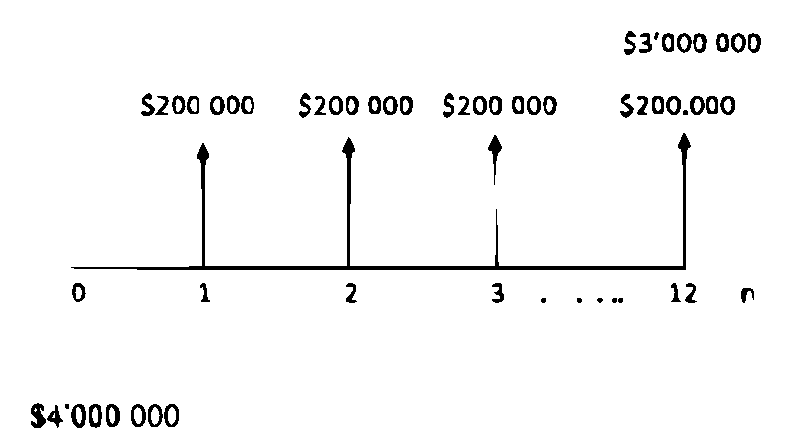
\includegraphics[scale=0.6, trim=-5 -5 -5 -5]{ejemplo7a.pdf} }   
\\ 
\multicolumn{3}{|c|}{ 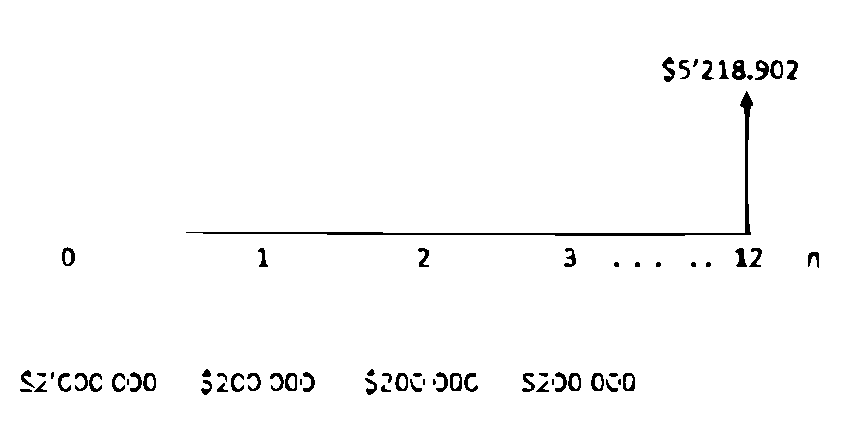
\includegraphics[scale=0.6, trim=-5 -5 -5 -5]{ejemplo7b.pdf} }   
\\ 
\hline
		%%%%%%%%%%%%% FIN INSERCIÓN DE IMAGEN
		%%%%%FIN FLUJO DE CAJA
		
		
		
		%%%%% INICIO DECLARACIÓN FORMULAS
		%%%%%%%%%%% INICIO TITULO
\rowcolor[HTML]{FFB183}
\multicolumn{3}{|c|}{\cellcolor[HTML]{FFB183}\textbf{4. Declaración de fórmulas}}    \\ \hline
		%%%%%%%%%%% FIN TITULO
		%%%%%%%%%%% INICIO MATEMÁTICAS
\multicolumn{3}{|c|} {VPN =	$\sum F_{n}(1+i)^{-n}$   Valor presente neto.}   \\ \hline	
	
		%%%%%%%%%% FIN MATEMÁTICAS
		%%%%%% INICIO DESARROLLO MATEMÁTICO
\rowcolor[HTML]{FFB183}
		%%%%%%%%%%INICIO TITULO
\multicolumn{3}{|c|}{\cellcolor[HTML]{FFB183}\textbf{5. Desarrollo matemático}}       \\ \hline
		%%%%%%%%%% FIN TITULO
		%%%%%%%%%% INICIO MATEMÁTICAS
		\multicolumn{3}{|c|}{$ \text{En la primera alternativa la financiera X le produce el 33\% naav} $}  
		\\
		
		\multicolumn{3}{|c|}{$ \text{sobre el total de su capital ( COP  6.000.000)} $}  
		\\
		\multicolumn{3}{|c|}{$ \text{mientras que en la segunda alternativa podrá comprar la máquina}$}  
		\\
		\multicolumn{3}{|c|}{$ \text{y le sobrarán  COP  2.000.000 que podrá invertir en la financiera.}$}  
		\\
		\multicolumn{3}{|c|}{$ \text{Y, además cada vez que la máquina le produzca un ingreso podrá} $}  
		\\
		\multicolumn{3}{|c|}{$ \text{ser reinvertido en la financiera Y. Esta segunda} $}  
		\\
		\multicolumn{3}{|c|}{$ \text{alternativa podría considerarse como formada por dos proyectos} $}  
		\\
		\multicolumn{3}{|c|}{$ \text{así:} $}  
		\\
		\multicolumn{3}{|c|}{$  COP  2.000.000(1+0.02)^{12} + COP  2.000.000(1+0.02)^{12} ..... =  COP  5.218.902 $}  
		\\
		\multicolumn{3}{|c|}{$ \text{Al fusionar el primero y el segundo proyecto en uno solo se} $}  
		\\
		\multicolumn{3}{|c|}{$\text{obtiene un tercer proyecto con egresos de  COP  6.000.000}$}  
		\\
		\multicolumn{3}{|c|}{$\text{( COP  4.000.000 +  COP  2.000.000) y con ingresos de  COP  8.218.902}$}
		\\
		\multicolumn{3}{|c|}{$ \text{que resultan de la suma de  COP  3.000.000 +  COP  5.218.902} $}  
		\\
		\multicolumn{3}{|c|}{ 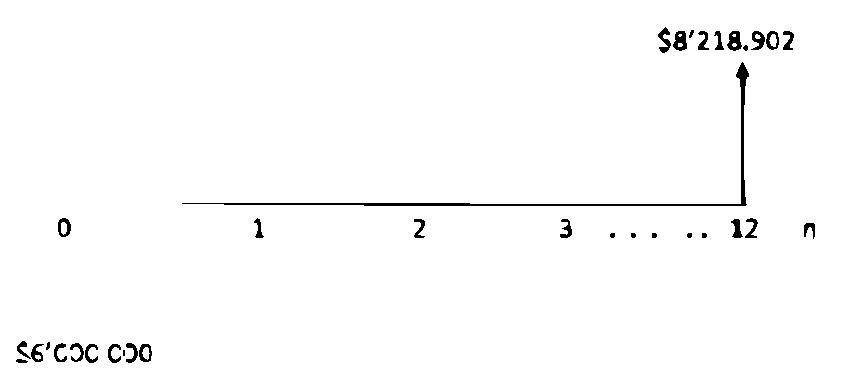
\includegraphics[scale=0.6, trim=-5 -5 -5 -5]{ejemplo7c.pdf} }   
		\\ 
		\multicolumn{3}{|c|}{$ \text{A este tercer proyecto se le puede calcular una tasa la cual}$}  
		\\
		\multicolumn{3}{|c|}{$\text{viene a ser TIR+R puesto que incluye reinversión y solo usamos}$}
		\\
		\multicolumn{3}{|c|}{$\text{una tasa que es la de reinversión.}$}
		\\
		\multicolumn{3}{|c|}{$\text{La tasa de este último proyecto la calcularemos anual para }$}
		\\ 
		\multicolumn{3}{|c|}{$\text{compararla con la primera alternativa. }$}
		\\ 		
		\multicolumn{3}{|c|}{$  COP  8.218.902 =  COP  6.000.000(1 + i)^{1}$}
		\\ 	
	    \hline
				
		%%%%%%%%%% FIN MATEMÁTICAS
		%%%%%% FIN DESARROLLO MATEMÁTICO
		%%%%%% INICIO RESPUESTA
\rowcolor[HTML]{FFB183}
		%%%%%%%%%%INICIO TITULO
\multicolumn{3}{|c|}{\cellcolor[HTML]{FFB183}\textbf{5. Respuesta}}   \\ \hline
		%%%%%%%%%% FIN TITULO
		%%%%%%%%%% INICIO RESPUESTA MATEMÁTICA
		
\multicolumn{3}{|c|}{ \text{Al despejar i se obtiene el 36.98\% naav y se concluye que es}}
\\
\multicolumn{3}{|c|}{\text{mejor la segunda alternativa que la primera que solo da el 33\% naav. } }
\\
\hline

		
		%%%%%%%%%% FIN MATEMÁTICAS
		%%%%%% FIN RESPUESTA
	\end{longtable}
	%Se crean dos lineas en blanco para que no quede el siguiente texto tan pegado
	%\newline \newline %USARLO SI CREES QUE ES NECESARIO
\end{center}
%%%%%%%%%%%%%%%%%%%%%%%%%%FIN EJERCICIO 1 %%%%%%%%%%%%%%%%%%%%%%%%%%%


\textbf{}\\
